\chapter{Opis implementacji}
\label{ImplementationChapter}
System stworzony na potrzebę realizacji niniejszej pracy magisterskiej można podzielić na dwa moduły, zgodnie z opisem architektury zamieszczonym w sekcji \ref{SoftwareArchSection}:
\begin{enumerate*}
\item Środowisko Uczenia - stworzone w silniku Unity i odpowiedzialne za symulowanie wirtualnego środowiska, po którym przemieszcza się inteligentny agent.
\item Narzędzie \texttt{mlagents\_learn} - wchodzi w skład zestawu \textit{Unity ML-Agents} (por. \ref{UnityMlSection}) i odpowiada za trening sieci konwolucyjnych. Jest procesem niezależnym od silnika Unity, a komunikacja ze Środowiskiem Uczenia odbywa się poprzez specjalny mechanizm, którego implementacja pochodzi z tego samego zestawu narzędziowego.
\end{enumerate*}

W dalszej części rozdziału znajduje się szczegółowy opis każdego z modułów.

\section{Środowisko Uczenia}
Jest typowym projektem stworzonym na silniku Unity, a w jego skład wchodzi wiele katalogów i plików. W tym rozdziale autor pracy skupił uwagę na opisanie jedynie najważniejszych elementów potrzebnych do zrozumienia aplikacji, zakładając że resztę informacji czytelnik pracy może pozyskać z dokumentacji silnika, stanowiącej bardzo dobre źródło wiedzy o tym narzędziu.

\subsection{Wykorzystane assety}
Assety to komponenty przeznaczone do wykorzystania w projektach uruchamianych na silniku Unity. Assety mogą być zasobami różnych typów, począwszy od modeli 3D i plików audio, a skończywszy na skryptach języka C\#. W ramach silnika Unity udostępniana jest specjalna usługa o nazwie \textit{Unity Asset Store} \cite{unity:assetStore}, która zapewnia dostęp do darmowych i płatnych assetów.

W realizowanym projekcie jest wykorzystywanych kilka paczek assetów, lecz najważniejsze z nich są dwa: \textbf{Environmental Race Track Pack} oraz \textbf{Vehicle Physics Pro}, którego dokładny opis zamieściłem w sekcji \ref{VppSection}.

\subsubsection{Environmental Race Track Pack}
Darmowa paczka, w skład której wchodzą cztery odmienne tory wyścigowe złożone z relatywnie małej liczby trójkątów \cite{unityAssets:envRaceTrackPack}:
\vspace{-0.5cm}
\begin{itemize*}
\item ,,\textit{Coastal Race Track}'' - tor nadbrzeżny,
\item ,,\textit{F1 Race Track}'' - tor Formuły 1,
\item ,,\textit{Racing Oval}'' - tor w kształcie owalnym,
\item ,,\textit{Figure 8 Track}'' - tor w kształcie ósemki.
\end{itemize*}
Na potrzeby implementacji systemu wykorzystano dwa tory z tej paczki, co dokładniej jest opisane w sekcji \ref{RaceTracksSection}.

\subsubsection{Vehicle Physics Pro}
Dokładny opis tego zestawu został zamieszczony w sekcji \ref{VppSection}, tutaj natomiast należy wspomnieć o najważniejszym z wykorzystanych assetów, czyli samochodzie \textbf{Sport Coupe}. Jest to dokładnie odwzorowany model 3D samochodu sportowego, posiadający skonfigurowaną fizykę jazdy. \textbf{Sport Coupe} jest jednym z dwóch skonfigurowanych modeli samochodów, dołączanych do zestawu Vehicle Physics Pro. Drugim z nich jest \textbf{JPickup}, czyli model samochodu typu pickup. Obydwa modele zostały zaprezentowane na rysunku \ref{VppCarModels}. \\

\begin{figure}[h]
\begin{center}
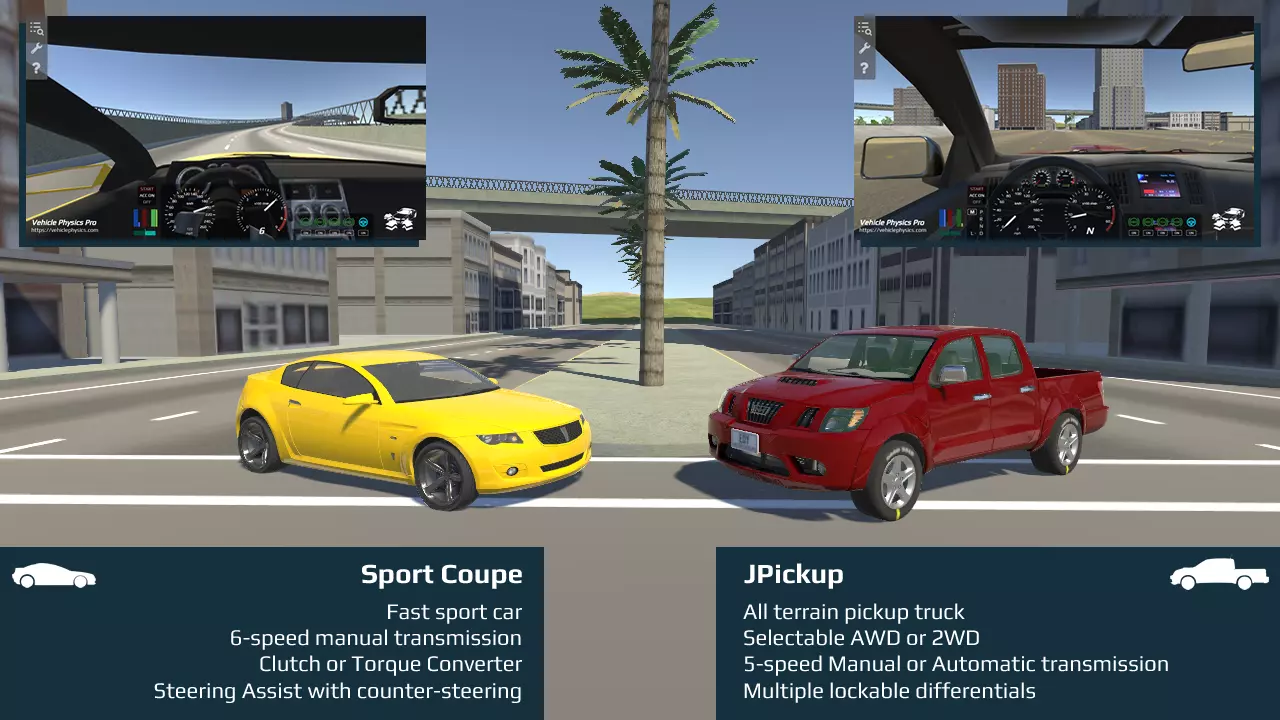
\includegraphics[width=14cm]{resources/figures/vpp-car-models.png}
\caption{Modele samochodów dostarczane w pakiecie Vehicle Physics Pro}
\source{https://assetstore.unity.com/packages/tools/physics/vehicle-physics-pro-community-edition-153556}
\label{VppCarModels}
\end{center}
\end{figure}

\newpage
\subsection{Tory wyścigowe}
\label{RaceTracksSection}
Na potrzeby implementacji systemu wykorzystano dwa tory z pakietu \textbf{Environmental Race Track Pack}: ,,\textit{Figure 8 Track}'' oraz ,,\textit{Coastal Race Track}''. Tory uległy delikatnym modyfikacjom, polegającym przede wszystkim na usunięciu niepotrzebnych elementów sceny oraz zmianie jej oświetlenia. Widok torów z lotu ptaka został uwieczniony na rysunku \ref{RaceTracksFig}. \\

\begin{figure}[h]
\begin{center}
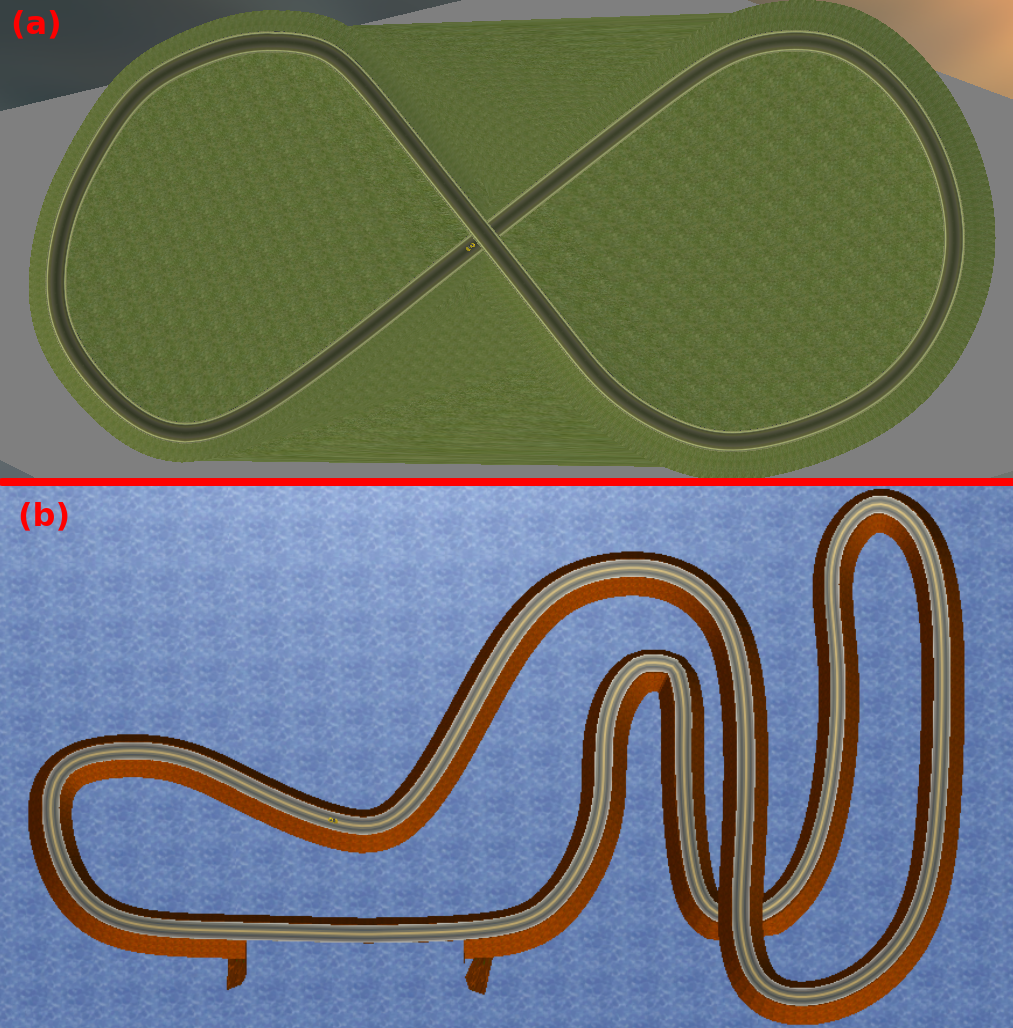
\includegraphics[width=14.5cm]{resources/figures/race_tracks_marked.png}
\caption{Tory wyścigowe wykorzystane w projekcie.}
\vspace*{-0.3cm}
\caption*{(a) Tor nr 1 - zmodyfikowany ,,\textit{Figure 8 Track}''}
\vspace*{-0.3cm}
\caption*{(b) Tor nr 2 - zmodyfikowany ,,\textit{Coastal Race Track}''}
\label{RaceTracksFig}
\end{center}
\end{figure}

\vspace{-0.5cm}
Tory różnią się od siebie przede wszystkim poziomem trudności - tor nr 2 wymaga od kierowcy znacznie większych umiejętności, ponieważ zakręty są bardziej zróżnicowane.

\subsection{Konfiguracja sceny Unity}
Na potrzeby eksperymentów obliczeniowych przygotowano kilka scen Unity. Zasadniczo różnią się one detalami, które dokładniej zostaną przedstawione w rozdziale \ref{ExperimentsChapter}-tym, natomiast ich rdzeń jest wszędzie taki sam. Najważniejszym obiektem na scenie jest \texttt{CarAgent}, reprezentujący model samochodu sterowany przez sieć neuronową. Obiekt składa się z kiku komponentów, wśród których najważniejsze to:
\vspace{-0.5cm}
\begin{enumerate*}
\item \textbf{Vehicle Controller} - komponent importowany z zestawu Vehicle Physics Pro (por. \ref{VppSection}). Odpowiada za ustawienia fizyki kluczowych elementów samochodu, takich jak: układ kierowniczy, hamulce, opony i skrzynia biegów \cite{vpp:vehicleController}. Na potrzeby implementacji systemu wprowadzono następujące zmiany w konfiguracji komponentu:
\begin{itemize*}
\item Zmiana skrzyni biegów na automatyczną oraz wyzerowanie wartości parametrów ,,\textit{Gear transition time}'' oraz ,,\textit{Shift interval}'';
\item Wyłączenie wspomagania kierownicy i systemów wspomagania jazdy: kontroli trakcji (TCS), kontroli stabilności (ESC) oraz zapobiegania nadmiernemu uślizgowi kół (ASR).
\end{itemize*}
\item \textbf{Behavior Parameters} - komponent importowany z zestawu Unity ML-Agents (por. \ref{UnityMlSection}). Jego celem jest określenie wartości dla kluczowych parametrów trenowanego zachowania, takich jak rozmiar wektora obserwacji oraz rozmiar wektora akcji. Wartości te ulegały zmianie dla poszczególnych eksperymentów obliczeniowych, dlatego ten aspekt implementacji zostanie dokładniej opisany w kolejnym rozdziale.
\item \textbf{Klasa dziedzicząca po klasie Agent} - skrypt C\#, w którym zawarto implementację klasy dziedziczącej po klasie \texttt{Agent}, wywodzącej się z zestawu Unity ML-Agents. Na potrzeby eksperymentów obliczeniowych przygotowano kilka wersji implementacji tego skryptu, jednak rdzeń odpowiedzialności pozostaje taki sam. Skrypt jest odpowiedzialny za: prawidłową inicjalizację każdego epizodu treningu, przekazywanie obserwacji ze Środowiska Uczenia do sieci neuronowej, przekazywanie wyjścia z sieci neuronowej do Środowiska Uczenia oraz obliczanie wartości sygnałów nagrody dla danego kroku symulacji. Oprócz tego, każda wersja implementacji posiada własne, dodatkowe odpowiedzialności.
\item \textbf{Decision Requester} - komponent importowany z zestawu Unity ML-Agents. Jego głównym zadaniem jest określenie częstotliwości podejmowania decyzji przez Agenta.
\item \textbf{Camera Sensor} - czujnik kamery, importowany z zestawu Unity ML-Agents. Jest niezbędny, jeśli chcemy dostarczać sieci neuronowej obserwacji wizualnych ze środowiska. Parametrami komponentu są m.in. wymiary obrazu oraz typ kompresji.
\end{enumerate*}

\clearpage
\section{Narzędzie mlagents\_learn}
Główne narzędzie do treningu sieci neuronowych, oferowane przez zestaw Unity ML-Agents \cite{unitymla:trainingMlAgents}. Parametry są przekazywane do narzędzia poprzez wiersz poleceń oraz plik konfiguracyjny utrzymany w formacie YAML \cite{unitymla:configFile}. Zestaw ustawień oraz hiperparametrów zdefiniowanych w pliku konfiguracyjnym zależy w ogromnym stopniu od zastosowanej metody treningowej oraz sposobu konfiguracji Środowiska Uczenia. Konkretna zawartość wykorzystanych plików konfiguracyjnych zostanie zaprezentowana w kolejnym rozdziale.

Wywołanie narzędzia skutkuje uruchomieniem procesu treningowego oraz rozpoczęciem uczenia sieci. W wyniku swojej pracy, proces treningowy generuje trzy artefakty:
\begin{enumerate*}
\item \textbf{Podsumowania} - metryki treningowe, aktualizowane podczas trwania treningu. Są bardzo pomocne przy monitorowaniu wyników uczenia sieci oraz ewentualnych aktualizacjach wartości hiperparametrów. Podsumowania można wyświetlić w eleganckiej formie graficznej, wykorzystując w tym celu narzędzie \textit{TensorBoard} \cite{unitymla:tensorboard}.
\item \textbf{Modele} - katalog z punktami kontrolnymi modelu aktualizowanego podczas szkolenia, a także ostateczny plik modelu. Plik ostateczny jest generowany jednorazowo, czyli po zakończeniu lub przerwaniu uczenia. Wszystkie wygenerowane modele są plikami w formacie ONNX \cite{onnx:website}.
\item \textbf{Pliki timerów} - zawierają zagregowane metryki procesu uczenia, w tym czas spędzony na określonych blokach kodu. Są bardzo pomocne podczas prac nad poprawą wydajności obliczeń procesu uczenia.
\end{enumerate*}

\subsection*{Trening sieci}
Podczas wszystkich eksperymentów obliczeniowych wykorzystywałem do treningu sieci metodę uczenia maszynowego o nazwie \textbf{uczenie ze wzmocnieniem} (z ang. \textit{reinforcement learning}). Zestaw narzędziowy Unity ML-Agents dostarcza implementacji dla dwóch algorytmów wspierających tę metodę - PPO \cite{ppo:opis} oraz SAC \cite{sac:opis}. Po kilku próbach okazało się, że do realizacji tematu pracy znacznie lepiej sprawdzi się algorytm PPO, dlatego właśnie on został wykorzystany we wszystkich eksperymentach obliczeniowych opisanych w rozdziale \ref{ExperimentsChapter}-tym. PPO jest wyjątkowe pośród innych algorytmów uczenia ze wzmocnieniem, ponieważ zachowuje balans pomiędzy łatwością implementacji, złożonością próbki oraz łatwością dostrajania. Z tego też powodu jest oferowany jako domyślny algorytm uczenia ze wzmocnieniem dla zestawu Unity ML-Agents.